% urban-short-report.tex
% v0.1 Sept. 2021

\documentclass{urban-formatting}

% New commands ---------------------------
\usepackage{amsmath, amssymb, amsthm, amsbsy, amsfonts, cases}
\usepackage[noend]{algpseudocode}
\usepackage[mathscr]{euscript}

\renewcommand*{\thefootnote}{\arabic{footnote}}
\renewcommand{\qedsymbol}{$\blacksquare$}
\newcommand{\bs}{\boldsymbol}
\newcommand{\M}{\mathcal{M}}
\newcommand{\R}{\mathcal{R}}
\newcommand{\T}{\mathcal{T}}
\newcommand{\x}{\mathbf{x}}
\newcommand{\z}{\mathbf{z}}
\newcommand{\w}{\mathbf{w}}
\newcommand{\s}{\mathbf{s}}
\newcommand{\e}{\mathbf{e}}
\newcommand{\vv}{\mathbf{v}}
\newcommand{\Lap}{\mathcal{LAP}}
\newcommand{\Exp}{\mathcal{EXP}}
\newcommand{\E}{\mbox{E}}

% Algorithms Stuff------------------------------
\theoremstyle{plain}
\newtheorem{thm}{Theorem}
\newtheoremstyle{exampstyle}
  {\topsep} % Space above
  {\topsep} % Space below
  {} % Body font
  {} % Indent amount
  {\bfseries} % Theorem head font
  {} % Punctuation after theorem head
  {.5em} % Space after theorem head
  {} % Theorem head spec (can be left empty, meaning `normal')
 
\newtheorem{defn}{Definition}
\newtheoremstyle{exampstyle}
  {\topsep} % Space above
  {\topsep} % Space below
  {} % Body font
  {} % Indent amount
  {\bfseries} % Theorem head font
  {.} % Punctuation after theorem head
  {.5em} % Space after theorem head
  {} % Theorem head spec (can be left empty, meaning `normal')
  
\providecommand{\keywords}[1]
{
  \small	
  \textbf{\textit{Keywords---}} #1
}

\usepackage{algpseudocode}
\usepackage{algorithm}
\algnewcommand\algorithmicinput{\textbf{Input:}}
\algnewcommand\Input{\item[\algorithmicinput]}
\algnewcommand{\algorithmicoutput}{\textbf{return:}}
\algnewcommand\Output{\item[\algorithmicoutput]}
\algnewcommand\algorithmicforeach{\textbf{for each}}
\algdef{S}[FOR]{ForEach}[1]{\algorithmicforeach\ #1\ \algorithmicdo}

\theoremstyle{plain}
\newtheorem{theorem}{Theorem}[section]
\newtheorem{corollary}{Corollary}[theorem]
\newtheorem{lemma}{Lemma}[theorem]
\newtheorem{proposition}{Proposition}[section]

% Default Stuff ---------------------------
% Font and Font Weight 
\usepackage[default]{lato}
\usepackage[T1]{fontenc}

% Setting the references list
\bibliography{references}

% Change out report title - use shortened title if necessary
\title{Differentially Private Methods for Validation Servers}

\begin{document}
% Setting the page numbering to be roman first
\pagenumbering{roman}


%%%%%%%%%%%%%%%%%%%%%%%%%%%%%%%%%%%% Title %%%%%%%%%%%%%%%%%%%%%%%%%%%%%%%%%%%%%%%%%

\begin{titlepage}
    % Add Policy Center/Intaitive/Toxonmy Term Bar
    % note the textbox exceeds width of document to avoid white space on sides
    \begin{textblock*}{9in}(-0.25in, 0.125in)
        \begin{tcolorbox}[valign = center]
            \begin{center}
                \policycenter{Technology and Data Science}
            \end{center}
        \end{tcolorbox}
    \end{textblock*}

    % Adding the cover image - code forces the image to be width of full paper (ignoring margins)
    \vspace*{-1.75cm}
    \noindent
    \makebox[\textwidth]{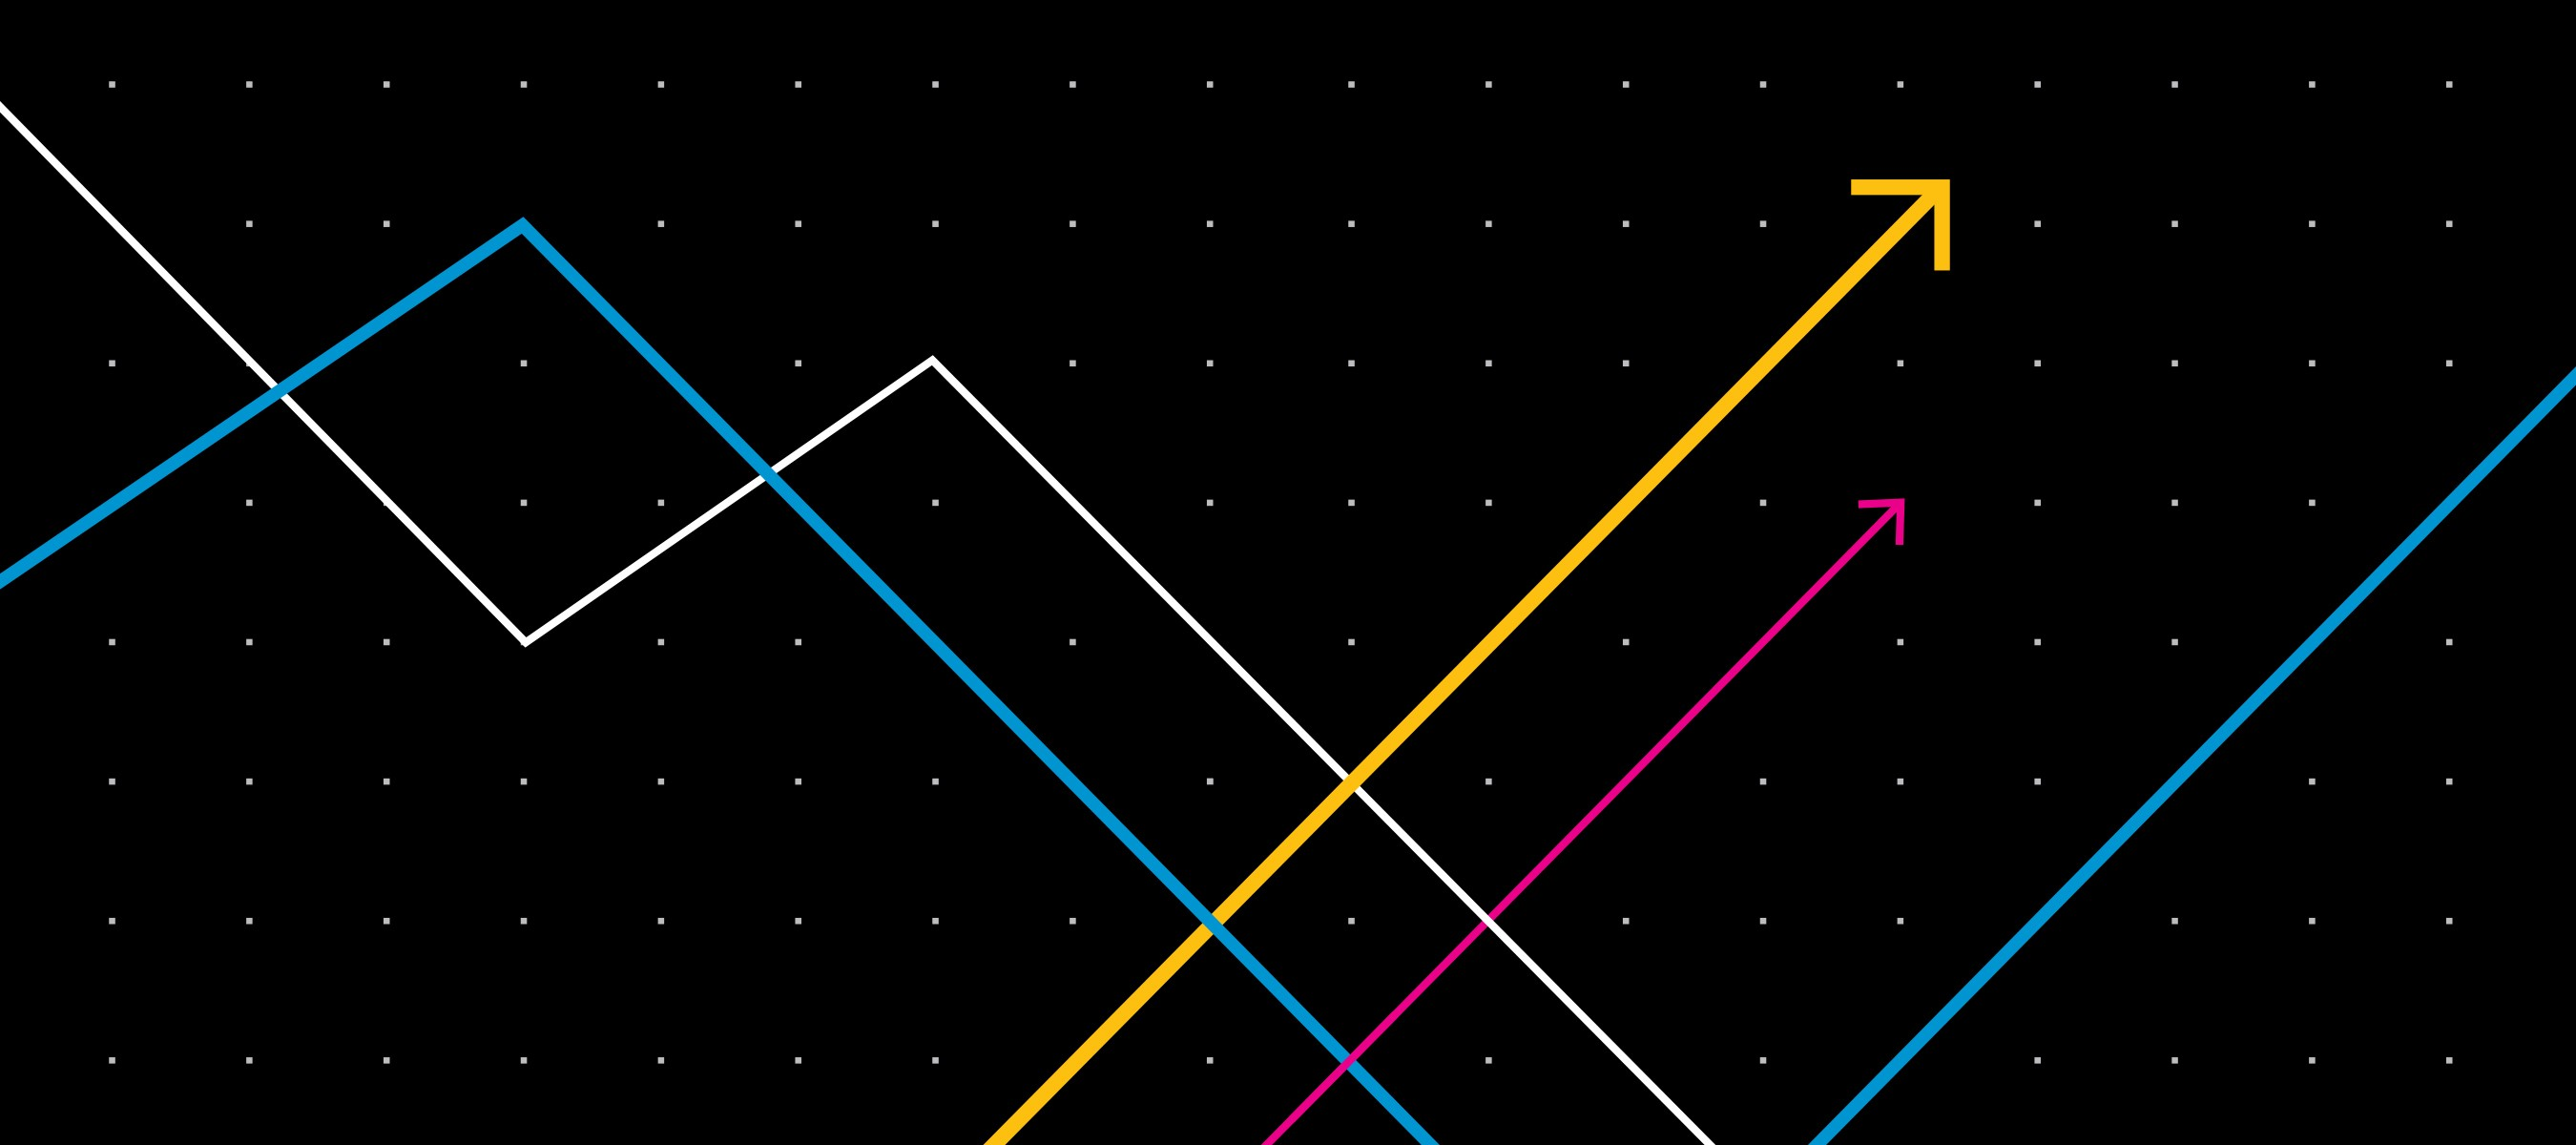
\includegraphics{images/cover.jpg}}
    
    \vspace{0.3in}
    \noindent\textcolor{urban-blue}{\MakeUppercase{\textbf{\so{Research Report}}}}
    
    \vspace{0.3in}
    \titlereport{Differentially Private Methods for Validation Servers}
    
    \reportsubtitle{A Feasibility Study of Differentially Private Summary Statistics and Regression Analyses for Administrative Tax Data}

    % Multiple column author names - change the "4" to the number of desired columns
    \begin{multicols}{4}
        \authorfont{Andr\'es F. Barrientos}\\
        \affiliationfont{Florida State University}
        
        \authorfont{Aaron R. Williams}\\
        \affiliationfont{Urban Institute}
        
        \authorfont{Joshua Snoke}\\
        \affiliationfont{RAND Corporation}
        
        \authorfont{Claire McKay Bowen}\\
        \affiliationfont{Urban Institute}
    \end{multicols}
    
    \vspace{-0.5cm}
    
    \datefont{September 2021}
    \vfill
    \vfill
    \vfill
    
    % Add logo
    \begin{textblock*}{4.5in}[1, 1](5.5in, 10.5in)
        \noindent
\includegraphics[width=4.5in]{images/cover-footer.jpg}
    \end{textblock*}
\end{titlepage}

%%%%%%%%%%%%%%%%%%%%%%%%%%%%%%%%%%%% About Urban %%%%%%%%%%%%%%%%%%%%%%%%%%%%%%%%%%%
%%%%%%%%%%%%%%%%%%%%%%%%%%%%%%%%%%%% About Urban %%%%%%%%%%%%%%%%%%%%%%%%%%%%%%%%%%%
\thispagestyle{empty} % Removed Page Number
\begin{figure}
    
\includegraphics[width=1.5in]{images/logo.png}
\end{figure}
\vspace*{-0.5in}
\about{About the Urban Institute}\\
\vspace{-5pt}
\boilerplate{The nonprofit Urban Institute is a leading research organization dedicated to developing evidence-based insights that improve people’s lives and strengthen communities. For 50 years, Urban has been the trusted source for rigorous analysis of complex social and economic issues; strategic advice to policymakers, philanthropists, and practitioners; and new, promising ideas that expand opportunities for all. Our work inspires effective decisions that advance fairness and enhance the well-being of people and places.}

\vspace*{\fill}
\begin{singlespace}
    \noindent Copyright © September 2021. Urban Institute. Permission is granted for reproduction of this file, with attribution to the Urban Institute. Cover image by Tim Meko.
\end{singlespace}

%%%%%%%%%%%%%%%%%%%%%%%%%%%%%%%%%%%% Table of Contents %%%%%%%%%%%%%%%%%%%%%%%%%%%%%
% Clears page and starts new page
\cleardoublepage

% Set page number to include title page
\setcounter{page}{3}
\begin{singlespace}
    \tableofcontents
\end{singlespace}

% Removed Page Number, must come after \tableofcontents
\thispagestyle{empty} 

%%%%%%%%%%%%%%%%%%%%%%%%%%%%%%%%%%%% Front Matter %%%%%%%%%%%%%%%%%%%%%%%%%%%%%%%%%%

% Footer Formatting: DO NOT CHANGE -----------------------------------
\fancyfoot{}

\fancyfoot[LE]{\colorbox{urban-footergray}{\makebox(0.2, 0.12)[r]{\fontsize{7.5}{0}\selectfont\bfseries{\MakeUppercase{}\hspace{0.2in}}}}\colorbox{urban-gold}{\makebox(0.2, 0.12)[c]{\fontsize{7.5}{0}\selectfont\bfseries{\MakeUppercase\thepage}}}\colorbox{urban-footergray}{\makebox(5.64, 0.12)[r]{\fontsize{7.5}{0}\selectfont\bfseries{\MakeUppercase{\so{Acknowledgments}}\hspace{0.2in}}}}}

\fancyfoot[RO]{\colorbox{urban-footergray}{\makebox(5.64, 0.12)[l]{\fontsize{7.5}{0}\selectfont\bfseries{\hspace{0.2in}\MakeUppercase{\so{Acknowledgments}}}}}\colorbox{urban-gold}{\makebox(0.2, 0.12)[c]{\fontsize{7.5}{0}\selectfont\bfseries{\MakeUppercase\thepage}}}\colorbox{urban-footergray}{\makebox(0.2, 0.12)[r]{\fontsize{7.5}{0}\selectfont\bfseries{\MakeUppercase{}\hspace{0.2in}}}}}

%%%%%%%%%%%%%%%%%%%%%%%%%%%%%%%%%%%% Acknowledgments %%%%%%%%%%%%%%%%%%%%%%%%%%%%%%%%%%%%
\part{Acknowledgments}

This report was funded by the Alfred P. Sloan Foundation and National Science Foundation National Center for Science and Engineering Statistics. We are grateful to them and to all our funders, who make it possible for Urban to advance its mission. 

The views expressed are those of the authors and should not be attributed to the Urban Institute, its trustees, or its funders. Funders do not determine research findings or the insights and recommendations of Urban experts. Further information on the Urban Institute’s funding principles is available at \href{https://www.urban.org/aboutus/our-funding/funding-principles}{urban.org/fundingprinciples}.

We would like to thank our collaborators at the Internal Revenue Service Statistics of Income Division, especially Barry Johnson and Victoria Bryant, for their amazing support for this project. We also thank our stellar validation server project team, consisting of Leonard Burman, John Czajka, Surachai Khitatrakun, Graham MacDonald, Rob McClelland, Silke Taylor, Kyle Ueyama, Doug Wissoker, and Noah Zwiefel. Thank you to Gabriel Morrison for reviewing our code.

Finally, we thank our advisory board, who have provided invaluable advice throughout the course of this project. The members are John Abowd, Jim Cilke, Jason DeBacker, Nada Eissa, Rick Evans, Dan Feenberg, Max Ghenis, Nick Hart, Matt Jensen, Barry Johnson, Ithai Lurie,  Shelly Martinez, Robert Moffitt, Amy O'Hara, Jerry Reiter, Emmanuel Saez, Wade Shen, Aleksandra Slavkovi\'c, Salil Vadhan, and Lars Vilhuber.

% Footer Formatting: DO NOT CHANGE -----------------------------------
\fancyfoot{}

\fancyfoot[LE]{\colorbox{urban-footergray}{\makebox(0.2, 0.12)[r]{\fontsize{7.5}{0}\selectfont\bfseries{\MakeUppercase{}\hspace{0.2in}}}}\colorbox{urban-gold}{\makebox(0.2, 0.12)[c]{\fontsize{7.5}{0}\selectfont\bfseries{\MakeUppercase\thepage}}}\colorbox{urban-footergray}{\makebox(5.64, 0.12)[r]{\fontsize{7.5}{0}\selectfont\bfseries{\MakeUppercase{\so{Executive Summary}}\hspace{0.2in}}}}}

\fancyfoot[RO]{\colorbox{urban-footergray}{\makebox(5.64, 0.12)[l]{\fontsize{7.5}{0}\selectfont\bfseries{\hspace{0.2in}\MakeUppercase{\so{Executive Summary}}}}}\colorbox{urban-gold}{\makebox(0.2, 0.12)[c]{\fontsize{7.5}{0}\selectfont\bfseries{\MakeUppercase\thepage}}}\colorbox{urban-footergray}{\makebox(0.2, 0.12)[r]{\fontsize{7.5}{0}\selectfont\bfseries{\MakeUppercase{}\hspace{0.2in}}}}}

%%%%%%%%%%%%%%%%%%%%%%%%%%%%%%%%%%%% Executive %%%%%%%%%%%%%%%%%%%%%%%%%%%%%%%%%%%%%%%%%
\part{Executive Summary}

\intropara{Federal tax data, derived from individuals' and businesses' tax and information returns, are invaluable resources for research on a range of topics. That research improves our understanding of individuals' and firms' responses to economic incentives. However, full access to these data is available only to select government agencies, to a very limited number of researchers working in collaboration with analysts in those agencies, or through highly selective programs within the Internal Revenue Service Statistics of Income Division. In addition, the existing process of manually vetting each statistical release for disclosure risks is labor intensive and imperfect because it relies on subjective human review.}
    
\intropara{As part of larger project to implement an automated validation server, we conduct an extensive feasibility study on several differentially private methods for releasing tabular statistics, mean and quantile statistics, and regression analyses. We provide a thorough discussion on which methods we tested and which methods could not be implemented in practice. We then evaluate the selected differentially private methods based on their impact on tax public policy decisions and several other utility metrics. From our findings, we outline the outstanding challenges and future work.}

%%%%%%%%%%%%%%%%%%%%%%%%%%%%%%%%%%%% Main Text %%%%%%%%%%%%%%%%%%%%%%%%%%%%%%%%%%%%%

% Footer Formatting: DO NOT CHANGE -----------------------------------
% Setting the page numbers to be arabic 
\pagenumbering{arabic}

\fancyfoot{}

\fancyfoot[LE]{\colorbox{urban-footergray}{\makebox(0.2, 0.12)[r]{\fontsize{7.5}{0}\selectfont\bfseries{\MakeUppercase{}\hspace{0.2in}}}}\colorbox{urban-gold}{\makebox(0.2, 0.12)[c]{\fontsize{7.5}{0}\selectfont\bfseries{\MakeUppercase\thepage}}}\colorbox{urban-footergray}{\makebox(5.64, 0.12)[r]{\fontsize{7.5}{0}\selectfont\bfseries{\MakeUppercase{\textls{\THETITLE}}\hspace{0.2in}}}}}

\fancyfoot[RO]{\colorbox{urban-footergray}{\makebox(5.64, 0.12)[l]{\fontsize{7.5}{0}\selectfont\bfseries{\hspace{0.2in}\MakeUppercase{\textls{\THETITLE}}}}}\colorbox{urban-gold}{\makebox(0.2, 0.12)[c]{\fontsize{7.5}{0}\selectfont\bfseries{\MakeUppercase\thepage}}}\colorbox{urban-footergray}{\makebox(0.2, 0.12)[r]{\fontsize{7.5}{0}\selectfont\bfseries{\MakeUppercase{}\hspace{0.2in}}}}}
% Footer Formatting: DO NOT CHANGE -----------------------------------
%%%%%%%%%%%%%%%%%%%%%%%%%%%%%%%%%%%% Report %%%%%%%%%%%%%%%%%%%%%%%%%%%%%%%%%%%%%
\part{Differentially Private Methods for Validation Servers}
\section{Introduction}\label{sec:intro}

Federal tax data, derived from individuals' and businesses' tax and information returns, are invaluable resources for research on a range of topics. That research improves our understanding of individuals' and firms' responses to economic incentives. Researchers can also use these data to study areas far removed from taxation. For example, \citet{chetty2014measuring} have used tax data to study economic mobility across generations and how elementary school teacher quality affects economic outcomes later in life \citep{chetty2011does}.

However, full access to these data is available only to select government agencies, to a very limited number of researchers working in collaboration with analysts in those agencies, or through highly selective programs within the Internal Revenue Service (IRS) Statistics of Income (SOI) Division. In addition, the existing process of manually vetting each statistical release for disclosure risks is labor intensive and imperfect because it relies on subjective human review. The tremendous demand to participate in such projects, which is limited by SOI resource constraints, indicates that much more high-quality research could be conducted if a safe and less resource-intensive method were developed to expand access.

\subsection{Background on Accessing Confidential Data}\label{subsec:background}
At the IRS, the current process to release analytic results on confidential datasets requires the researcher to undergo an extensive background check (IRS clearance) to access the data, and then, an IRS staff member must review any results the researcher wants to release. This process reflects the norm for researchers wishing to access federal confidential data. Researchers either gain access from a public use file that is an altered version of the confidential data or have direct access to the confidential data.

As a potential middle ground between the two extremes, the US Census Bureau provides research access to two experimental synthetic databases via the Synthetic Data Server at Cornell University: the Synthetic Longitudinal Business Database and the Survey of Income and Program Participation's Synthetic Beta Data Product \citep{benedetto2013creation,drechsler2014synthetic}. The Synthetic Data Server provides a validation server that allows researchers to submit their statistical programs to run on the underlying administrative data after testing it on the publicly available synthetic data.

However, the Synthetic Data Server has two disadvantages. First, because it is not automated, the process consumes limited staff time, which demand often exceeds. This situation causes long delays for approval. Second, reviews may be inconsistent because they are manually evaluated by humans and do not adhere to formal notions of privacy that constrain the allowable output.

To address these problems for a validation server, some privacy researchers have proposed using a newer privacy loss definition, differential privacy (DP), as a means to automate the process \citep{dwork2006calibrating}. DP emerged from the computer science community as a rigorous definition for privacy loss associated with data publishing. Since then, many data privacy experts regard DP as the gold standard for privacy protection. It is part of a larger class of approaches often called \textit{formally private} methods because statisticians can mathematically prove the privacy loss that would result from a data publication that uses differentially private methods.

DP differs from prior statistical disclosure control or limitation methods because it does not require a simulated attacker or the same strong assumptions concerning how much information an intruder may have or what kind of disclosure is likely to occur. This does not imply that DP protects from all attacks, but, for a defined type of privacy loss, it offers provable amounts of protection.

At a high level, DP links the potential for privacy loss to how much the answer of a query (such as a statistic) is changed given the absence or presence of the most extreme possible person or observation in the data population. DP requires that the level of protection is set proportionally to this maximum potential change, thereby providing formal privacy protections scaled to the worst-case scenario. For further details, \citet{dwork2014algorithmic} provide a rigorous mathematical review of DP. \citet{bowen2021philosophy} cover the basics of DP and its challenges for adoption geared toward a general, mathematical audience, whereas \citet{nissim2017differential} and \citet{snoke2019differential} describe DP for a nontechnical, general audience. 

In this report, we examine the feasibility of differentially private methods for our target analyses and more complex ones. Specifically, we highlight the general findings from our extensive feasibility study on several differentially private methods for releasing tabular statistics, mean and quantile statistics, and regression analyses with cross-sectional data \citep{barrientos2021}. Based on informal interviews and our tax expert collaborators, we prioritized these analyses for the first stage of the validation server. There are several other analyses, such as model selection, that have been identified as important but will be explored for later development stages of the validation server. Further, we outline the methodological and practical challenges for implementing differential privacy on more complex analyses, such as regression discontinuity design.

\subsection{Background on Differential Privacy}\label{subsec:dp}
Differential privacy (DP) offers a provable and quantifiable amount of privacy protection, colloquially referred to as the privacy loss budget. Those in the data privacy and confidentiality community should note that DP provides a statement about the algorithm (or mechanism), not the data---a common misconception. In other words, DP requires that the \textit{mechanism} or \textit{algorithm} produces an output that provably meets the definition. We refer to these methods as differentially private algorithms or mechanisms.

In this section, we reproduce the pertinent definitions and theorems of DP with the following notation: $X\in\mathbb{R}$ is the original dataset  with dimension ${n\times r}$ and $X^*$ is the private version of $X$ with dimension ${n^*\times r}$. We also define a statistical query as a function $u:\mathbb{R}^{n\times r}\rightarrow\mathbb{R}^k$, where the function maps the possible datasets of $X$ to $k$ real numbers.

\subsubsection{Definitions and Theorems}\label{subsec:def}
\begin{defn}\label{def:dp}
    \textbf{Differential Privacy} \citep{dwork2006calibrating}:
    A sanitization algorithm, $\M$, satisfies $\epsilon$-DP if for all subsets $S\subseteq Range(\M)$ and for all $X,X'$ such that $d(X,X')=1$, 
        \begin{equation}\label{eqn:dp}
            \frac{\Pr(\M( X) \in S)}{ \Pr(\M( X')\in S)}\le \exp(\epsilon)
        \end{equation}
    \noindent where $\epsilon>0$ is the privacy loss budget and $d(X,X')=1$ represents the possible ways that $X'$ differs from $X$ by one record.
\end{defn}
\vspace{-8pt}
Definition \ref{def:dp} provides what is known as $\epsilon$-DP. There are varying understandings of what it means to differ by one record. One interpretation is the presence or absence of a record, and the other has the difference as a change, where $X$ and $X'$ have the same dimensions. \citet{li2016differential} refers to these interpretations as \textit{unbounded DP} for addition or removal of a record and \textit{bounded DP} for the change of a record. They prove that unbounded DP satisfies an important composition theorem we will discuss later in this section (see Theorem \ref{thm:comp}), whereas bounded DP does not. Because many DP methods rely on Theorem \ref{thm:comp}, we assume unbounded DP in this paper.

Several relaxations of $\epsilon$-DP have been developed in order to inject less noise into the output, such as approximate DP \citep{dwork2006our}, probabilistic DP \citep{machanavajjhala2008privacy}, concentrated DP \citep{dwork2016concentrated}, R\'enyi differential privacy \citep{mironov2017renyi}, and zero-concentrated DP \citep{bun2016concentrated}. Though these definitions are still formally private, they offer slightly weaker privacy guarantees. In return, they typically lessen the amount of noise required. We will cover approximate DP, also known as $(\epsilon, \delta)$-DP, and zero-concentrated DP in depth, because most of the methods we test in our study use one of these two definitions.

\begin{defn}\label{def:adp} \textbf{$(\epsilon, \delta)$-Differential Privacy} \citep{dwork2006our}:
A sanitization algorithm, $\M$, satisfies $(\epsilon, \delta)$-DP if for all $X, X'$ that are $d(X,X')=1$,
    \begin{equation}\label{eqn:adp}
        \Pr(\M( X) \in S)\le \exp(\epsilon) \Pr(\M( X')\in S) + \delta
    \end{equation}
    where $\delta\in [0,1]$. $\epsilon$-DP is a special case of $(\epsilon, \delta)$-DP when $\delta=0$.
\end{defn}
\vspace{-8pt}
Definition \ref{def:adp} provides a simple relaxation of Definition \ref{def:dp} by adding the parameter $\delta$. This allows, with small probability, that the strict bound given does not hold, which can be useful when dealing with extreme yet very unlikely cases.

\cite{dwork2016concentrated} proposed concentrated DP, which aimed to reduce the privacy loss over multiple computations (more on composition of multiple queries soon when discussing Theorem \ref{thm:comp}).

This definition of privacy was later on improved by
\cite{bun2016concentrated} who introduced zero-concentrated DP (zCDP or $\rho$-zCDP), given in Definition \ref{def:scdp}. 
They also show in their Proposition 1.3 that if $M$ satisfies $\rho$-zCDP, then $M$ is $(\rho+2\sqrt{\rho\log(1/\delta)},\delta)$-DP for any $\delta>0$. For the other direction, their Proposition 1.4 states that if $M$ satisfies $\epsilon$-DP, then $M$ satisfies $(1/2\epsilon^2)$-zCDP, which allows us to relate $\rho$-zCDP algorithms to an $\epsilon$-DP equivalent.

\begin{defn}\label{def:scdp} \textbf{Zero-Concentrated Differential Privacy} \citep{bun2016concentrated}:
A sanitization algorithm, $\M$, satisfies $(\xi, \rho)$-zero-concentrated differential privacy if for all $X, X'$ that are $d(X,X')=1$ and $\alpha\in (1, \infty)$,
    \begin{equation}
        D_\alpha(\M(X)||\M(X'))\leq\xi+\rho\alpha,
    \end{equation}
    where $D_\alpha(\M(X)||\M(X'))$ is the $\alpha$-R\'enyi divergence
    between the distribution of $\M(X)$ and the distribution of $\M(X')$, $\xi$ and $\rho$ are positive constants, and $\alpha \in (1,\infty)$.
\end{defn}
\vspace{-8pt}
As mentioned before, many DP algorithms require repeated responses from a query system, such as a validation server. Each time a statistic or output is released, data information ``leaks'' and must be protected. DP protects the information by splitting the amount of $\epsilon$ used for each output, and the composition theorems formalize this concept.

\begin{thm}\label{thm:comp} \textbf{Composition Theorems} \citep{mcsherry2009privacy,dwork2016concentrated,bun2016concentrated}:
Suppose a mechanism, $\M_j$, provides $(\epsilon_j$, $\delta_j)$-DP or $(\xi_j,\rho_j)$-zCDP for $j=1,\ldots,J$.
  \begin{itemize}\setlength{\itemindent}{15pt}
  \item[a)] \textbf{Sequential Composition:} The sequence of $\M_j(X)$ applied on the same $X$ provides $(\sum_{j=1}^J\epsilon_j,\sum_{j=1}^J\delta_j)$-DP or $(\sum_{j=1}^J\xi_j,\sum_{j=1}^J\rho_j)$-zCDP.
  \item[b)] \textbf{Parallel Composition:} Let  $D_j$ be disjoint subsets of the input domain $D$. The sequence of $\M_j(X\cap D_j)$ provides $(\max_{j \in \{1,\ldots,J\}} \epsilon_j, \max_{j \in \{1,\ldots,J\}} \delta_j)$-DP or \\ $(\max_{j \in \{1,\ldots,J\}}\xi_j, \max_{j \in \{1,\ldots,J\}}\rho_j)$-zCDP.
  \end{itemize}
\end{thm}
\vspace{-8pt}
More simply, suppose there are $J$ many statistical queries on $X$. The composition theorems state that we may allocate a portion of the overall desired level of $\epsilon$ to each statistic by sequential composition. A typical appropriation is dividing $\epsilon$ equally by $J$. For example, a data practitioner might want to query the mean and standard deviation of a variable. These two queries will require using the sequential composition, allocating an equal amount of privacy budget to each query. Conversely, parallel composition does not require splitting the budget because the noise is applied to disjoint subsets of the input domain. Privacy experts will often leverage parallel composition, for instance, to sanitize histogram counts, where the bins are disjoint subsets of the data. In this example, noise can be added to each bin independently without needing to split $\epsilon$.

The post-processing theorem is another important theorem, which states that any function applied to a DP output also satisfies DP. Many DP methods use the post-processing theorem to correct any inconsistencies or values that are not possible and to compute additional summaries required to perform statistical inference.

\begin{thm}\label{thm:post} \textbf{Post-Processing Theorem} \citep{dwork2006calibrating,nissim2007smooth, bun2016concentrated}:
If $\M$ be a mechanism that satisfies $(\epsilon,\delta)$-DP or $(\xi,\rho)$-zCDP, and $g$ be any function, then $g\left(\M(X)\right)$ also satisfies $(\epsilon,\delta)$-DP or $(\xi,\rho)$-zCDP.
\end{thm}

\subsubsection{Differentially Private Mechanisms}\label{subsec:mech}
In this section, we present two of the fundamental mechanisms we consider that satisfy $\epsilon$-DP and $(\epsilon, \delta)$-DP. We employ additional mechanisms that will be discussed in Section \ref{sec:DPalgorithforTax}. For a given value of $\epsilon$ and $\delta$, an algorithm that satisfies DP or approximate DP will adjust the amount of noise added to the output based on the maximum possible change between two databases that differ by one row. This value is commonly referred to as the global sensitivity (GS), given in Definition \ref{def:gs}.
\begin{defn}\label{def:gs} \textbf{$l_1$-Global Sensitivity} \citep{dwork2006calibrating}:
For all $X,X'$ such that $d(X,X')=1$, the global sensitivity of a function $M$ is
    \begin{equation}\label{eqn:gs}
        \Delta_1 (M)= \underset{d(X,X')=1}{\text{sup}} \|M(X)-M(X') \|_1 
    \end{equation}
\end{defn}
\vspace{-8pt}
We can calculate sensitivity under different norms. For instance, $\Delta_2(M)$ represents the $l_2$ norm GS, $l_2$-GS, of the function $M$. Another way of thinking about the GS is that it measures the statistical query's robustness to outliers. Though the definition is straightforward, calculating the GS can often be difficult. For instance, we cannot directly calculate an upper bound for the GS of one of the most common statistical analyses, regression, where the coefficients are unbounded. To address this issue, privacy researchers had to be creative in figuring out how to add noise to regression analyses.

The most basic mechanism satisfying $\epsilon$-DP is the Laplace mechanism, given in Definition \ref{def:lap}, and was first introduced by \cite{dwork2006calibrating}. Another popular mechanism is the Gaussian mechanism that satisfies $(\epsilon, \delta)$-DP, given in Definition \ref{def:gauss}, which uses the $l_2$-GS of the statistical query.
\begin{defn}\textbf{Laplace mechanism} \citep{dwork2006calibrating}: \label{def:lap}
The Laplace mechanism satisfies $\epsilon$-DP by adding noise  $(\eta_1,\ldots,\eta_k)$ to $M$ that are independently drawn from a Laplace distribution with the location parameter at 0 and scale parameter of $\Delta_1(M)\epsilon^{-1}$ such that 
    \begin{equation}\label{eqn:lap}
        \M(X)=M(X)+(\eta_1,\ldots,\eta_k).
    \end{equation}
\end{defn}
\vspace{-8pt}
\begin{defn}\label{def:gauss} \textbf{Gaussian mechanism} \citep{dwork2014algorithmic}:
    The Gaussian mechanism satisfies $(\epsilon,\delta)$-DP by adding Gaussian noise with zero mean and variance, $\sigma^2$, such that
        \begin{equation}\label{eqn:gauss}
            \M(X)=M(X)+(\eta_1,\ldots,\eta_k)
        \end{equation}
    where $\eta_1,\ldots,\eta_k$ are independently drawn and $\sigma=\Delta_2(M)\epsilon^{-1} \sqrt{2 \log(1.25/\delta)}$. 
\end{defn}
\vspace{-8pt}
Although \cite{dwork2014algorithmic} proposed Gaussian mechanism for $(\epsilon,\delta)$-DP, the Gaussian mechanism satisfies $((\Delta_2(M))^2/2\sigma^2)$-zCDP, per Proposition 1.6 from \cite{bun2016concentrated}. Additionally, if the $l_2$-GS is 1 (which is true for all counting queries), then the Gaussian mechanism satisfies $\left(\alpha, \frac{\alpha}{2\sigma^2}\right)$-R\'enyi DP, per Corollary 3 from  \cite{mironov2017renyi}. We use this relationship for multiple counting queries to reduce the amount of noise being added from the Gaussian mechanism. 

Both the Laplace and Gaussian mechanisms are simple and quick to implement, but they apply only to numerical values (without additional post-processing, Theorem \ref{thm:post}). A more general $\epsilon$-DP mechanism is the Exponential mechanism, given in Definition \ref{def:exp}, which allows for the sampling of values from a noisy distribution rather than adding noise directly. 

 \begin{defn}\label{def:exp} \textbf{Exponential mechanism} \citep{mcsherry2007mechanism}:
     The Exponential mechanism releases values with a probability proportional to
         \begin{equation}\label{eqn:exp}
             \exp \left(\frac{\epsilon u(X, \theta)}{2\Delta_1(u)}\right)
         \end{equation}
     and satisfies $\epsilon$-DP, where $u(X,\theta)$ is the score or quality function that determines the values for each possible output, $\theta$, on $X$.
 \end{defn}
\vspace{-8pt}
\subsubsection{Determining the Privacy Loss Parameters}
The mechanisms reviewed provide levels of privacy protection determined by the value of privacy parameters, such as $\epsilon, \delta$, or $\rho$. For a validation server, the relative merits and interpretations for chosen values of these parameters would need to be understood and communicated to policymakers. It is also important to understand that when considering the total privacy loss budget, choosing the value of $\epsilon$ for any single query is sensitive to other factors, such as the sample size, the total number of desired queries, and the size of the population from which data are sampled (if sampled). Those questions concern the overall framework that would need to be created for a fully implemented validation server, and we do not seek to answer those questions at this stage.

We explore a wide range of $\epsilon$ and $\delta$ values for this study, ranging from ones seen in theoretical work to practical applications. By doing so, we will gain a better sense of the privacy-utility trade-off. Specifically, we will examine the affects of $\epsilon$ and $\delta$ on accuracy within the context of our study, which we hope will contribute to the conversation about how to set the privacy-loss budget.

\subsection{Tax Data Use Cases}\label{subsec:data}
When deciding the scope of the statistical analyses the validation server will cover, we interviewed six economists who specialize in taxation, econometrics and causal inference, and other fields that use tax data. They emphasized the importance of custom tabulations for their work, which one economist referred to as ``low-hanging fruit.'' Many recent journal articles using tax data relied on aggregated data. Examples include the ongoing analyses of income inequality \citep{auten2018income} and wealth inequality \citep{smith2019top}, the growth of gig work in the economy \citep{collins2019gig}, and decisions on retirement savings \citep{brady2020reconciling}.

Other researchers have used aggregations of data in linear regressions on topics such as the effects of attitudes toward government and tax evasion \citep{cullen2021political}, the effect of tax credits on the labor market \citep{tong2014impact} and optimal taxation \citep{piketty2014optimal}. Researchers have also used aggregated data to infer behavioral responses by examining bunching at kink points \citep{chetty2011adjustment} and notches \citep{kleven2013using} in the tax code. \citet{mortenson2020bunching}, for example, investigate bunching at kink points formed from the formula for computing earned income tax credits.

With these analyses in mind, we tested the differentially private methods on the IRS SOI public use file (PUF) \citep{barrientos2021}. This is a database of sampled individual income tax returns with privacy protections applied that is developed and released annually by IRS SOI. Several organizations, such as the American Enterprise Institute, the Urban-Brookings Tax Policy Center, and the National Bureau of Economic Research, develop PUF-based microsimulation models that help inform the public on potential impacts of policy proposals. But access to this public file is limited to certain institutions, and we cannot provide the full data. For this reason, we also test on the 1994 to 1996 Current Population Survey Annual Social and Economic Supplements, accessed through IPUMS USA \cite{ruggles2021cps}, a publicly available dataset. Crucially, it has similar variables as the PUF, and the case study results on the Current Population Survey will be similar to those run on the IRS SOI.

A tax expert would likely query the following as exploratory data analysis before statistical modeling, which we based our feasibility study on:

\begin{itemize}
    \item \textbf{Single counting query}: How many tax returns have salary and wage income in excess of \$100,000?
    \item \textbf{Mean statistic query}: What are the means for the total population and subsets of the total population?
    \item \textbf{Quantile statistic query}: What is the income threshold for the top 10 percent of earners?
    \item \textbf{Regression query}: What effects do marginal tax rates have on capital investment?
\end{itemize}

\section{Tested Differentially Private Algorithms}\label{sec:dp-mech}
In this section, we survey differentially private methods we explored for the feasibility study and highlight the general results. We provide full details in \citet{barrientos2021}.

When testing our methods, we explored various values of $\epsilon$ and $\delta$. For the tabular, we set $\epsilon =\{0.01, 0.05, 0.1, 0.5, 1, 5, 10, 15, 20\}$ and $\delta=\{10^{-3},10^{-7},10^{-10}\}$. For the mean and quantile statistics, we set $\epsilon =\{0.1, 0.5, 1, 5, 10, 15, 20\}$ and $\delta=\{10^{-3},10^{-7},10^{-10}\}$. For the regression analyses, we set $\epsilon =\{0.5, 1, 5, 10, 15, 20\}$, $\delta=\{10^{-3},10^{-7},10^{-10}\}$. We based these values from what is seen in other practical applications and from our initial tests. We replicated all differentially private methods 100 times to assess variability.

\subsection{Tabular Statistics}
Researchers have fully developed differentially private tabular statistics. The literature already shows that adding Laplace noise produces the most accurate estimates for single tabular queries. For example, \citet{rinott2018confidentiality} found for disseminating frequency tables, the Laplace mechanism performed the best overall. Other DP research reports similar results because the Laplace mechanism is still ``hard to beat'' when the data have a large number of observations, or there are a lot of parameters and attributes to consider \citep{bowen2021differentially,shlomo2018statistical,liu2018generalized}.

Although the Gaussian mechanism produces wider tails, theory suggests adding Gaussian noise will perform better than adding Laplace noise for multiple counting queries because of how the tails compose \citep{wang2019subsampled}. We can improve this composition property by leveraging the R\'enyi differential privacy, which reduces the amount of noise added to each count. A drawback to using the Gaussian mechanism is that it satisfies $(\epsilon,\delta)$-DP, requiring the data user to balance two privacy parameters instead of one.

There are other differentially private algorithms that tackle more complex tabular statistics. However, the tax analyses we selected for the feasibility study are simple counting queries. This means we expect the Laplace and Gaussian mechanisms will meet our accuracy goals. Therefore, we do not choose to explore the more extensive differentially private tabular algorithms or apply any sophisticated postprocessing.

This brings up the question of why we tested the Laplace and Gaussian mechanisms for our study. Even though there is extensive literature, we still test the Laplace and Gaussian mechanisms for two reasons. First, we must verify these methods work well on our tax data. Second, the feasibility study can provide additional context for the privacy-utility trade-off in calculating an appropriate privacy loss budget.

In \citet{barrientos2021}, we confirmed that the Laplace mechanism outperformed the Gaussian mechanism, even for larger values of $\delta$. We note that both methods are unbiased, and for $\epsilon \geq 5$ they both perform well enough that there is little difference between them. Overall, these results suggest the Laplace mechanism would perform well enough to enable researchers to query accurate private histograms.

\subsection{Quantile Statistics}
The leading methods for generating differentially private quantiles use either the Laplace mechanism or the Exponential mechanism. For instance, \citet{smith2011privacy} proposed an algorithm, \textit{IndExp}, for selecting individual quantiles using the Exponential mechanism. \textit{IndExp} has since been implemented in the SmartNoise\footnote{"SmartNoise Differential Privacy Library," Microsoft, accessed July 20, 2021, https://github.com/opendp/smartnoise-core/tree/develop/whitepapers/mechanisms/exponential\_median.} and IBM DP libraries.\footnote{"IBM Differential Drivacy Library," GitHub, accessed July 20, 2021, https://github.com/IBM/differential-privacy-library/blob/main/diffprivlib/tools/quantiles.py.} This method was recently extended for querying multiple quantiles by \citet{gillenwater2021differentially} to two other algorithms, \textit{AppIndExp} and \textit{JointExp}. The former is the same as \textit{IndExp} but uses the composition theorem from \citet{dong2020optimal} to choose an optimal $\epsilon$ for multiple queries given a total ($\epsilon$, $\delta$), and the latter samples multiple quantiles jointly. \textit{JointExp} uses similar techniques to \textit{IndExp} but outputs multiple quantiles simultaneously. Using the Laplace mechanism, \citet{nissim2007smooth} developed an approach for sampling median values using smooth sensitivity that can be extended to query any other quantile. We will hereafter refer to this method as \textit{Smooth}. A few other approaches or adaptations of the approaches listed here have been proposed, but we did not test them because they require fine-tuning based on distribution assumptions that a researcher might not realistically have in our validation server setting.

In \citet{barrientos2021}, we found overall that both \textit{AppIndExp} and \textit{JointExp} offer high-quality quantiles, and they were generally preferable to \textit{Smooth} for all but the highest values of $\epsilon$. \textit{JointExp} performs better at estimating the zero-valued quantiles, though \textit{AppIndExp} offers high-quality performance at most levels of $\epsilon$ and $\delta$. Similarly, \textit{JointExp} has slightly lower relative bias on average for the nonzero quantiles, but the difference between the two algorithms is very small. 

For a practical validation server implementation, \textit{AppIndExp} and \textit{JointExp} both appear sufficient to return accurate quantile estimates. The choice would likely depend on whether the system deploys pure DP or approximate DP. We do not recommend that a system use \textit{Smooth} unless queries are made with very high levels of $\epsilon$. Additionally, we find that \textit{AppIndExp} returns more equally biased results for each quantile because they are drawn independently. On the other hand, \textit{JointExp} can return biased results, which are more biased for some quantiles than others because they are drawn from a noisy joint distribution.

In our application, the quantiles follow an exponential trend. \textit{JointExp} returns more accurate results for the lowest and highest quantiles but returns less accurate results for those in-between. It may be preferable to choose one or the other algorithm, depending on the application.

\subsection{Means and Confidence Intervals}
For mean estimates, we specifically reviewed differentially private methods that released means with their associated confidence intervals (CI). When we explored the general literature, we found common approaches use the Laplace mechanism, Gaussian mechanism, or Exponential mechanisms for releasing some means with CIs.

As with the quantiles, some methods require more information than is realistic for our application. For instance, \citet{karwa2017finite, bowen2020comparative, d2015differential, biswas2020coinpress} require the researcher to set bounds for the standard deviation to calculate the global sensitivity to add Laplace noise. In a validation server setting, a researcher might not have a good sense of the bounds. Given this limitation, we did not test them for our study.

\citet{du2020differentially} conducted a comprehensive research study that aimed to move the theory to practice for releasing differentially private CIs. The authors developed five new methods, two based on directly applying Laplace noise named \textit{NOISYVAR} and \textit{NOISYMAD} and three based on querying quantiles from the Exponential mechanism  to estimate the standard deviation named \textit{CENQ}, \textit{SYMQ}, and \textit{MOD}. \citet{du2020differentially} also compared their methods against \citet{karwa2017finite}; \citet{d2015differential}; and \citet{brawner2018bootstrap}. They found the two best performing for simulated Gaussian data were \textit{NOISYMAD} and \textit{SYMQ}. \textit{NOISYMAD} adds Laplace noise to the mean absolute deviation and the associated standard deviation, whereas \textit{SYMQ} computes two different quantiles that are equal distance away from the median and adds noise from the Exponential mechanism. A potential limitation to the approach using quantiles is that it strongly assumes the data are approximately Gaussian, since the confidence intervals are centered on the median rather than the mean. We chose not to test these methods on skewed data because preliminary tests showed extremely poor performance.

In \citet{barrientos2021}, the results show that the non-quantile-based methods are approximately unbiased. \textit{NOISYMAD} and \textit{NOISYVAR} perform similarly and both provide highly accurate statistics. BHM performs comparably to the other two methods only when $\delta = 0.01$ and when $\epsilon < 1$. Otherwise, the other two clearly outperform BHM.

For the associated confidence intervals, we find \textit{NOISYVAR} offers the best performance at all but the lowest level of $\epsilon$. \textit{NOISYMAD} performs well for very small values of $\epsilon$, but, as $\epsilon$ gets larger, the width of the CIs produced by \textit{NOISYMAD} shrinks and are consistently more narrow than the confidential CI. These results would produce overly confident inference for researchers making this query. Overall, \textit{NOISYVAR} is preferable, and it is capable of providing sufficiently accurate confidence intervals for all but the lowest levels of $\epsilon$.

\subsection{Regression Analyses}
In this section, we begin with an overview of the currently available differentially private approaches for regression analysis. We then explain the criteria for including methods in the feasibility study, where we discuss the selected methods and any adaptions made before inclusion in more detail.

\subsubsection{Traditional Differentially Private Approaches for Regression Analyses}\label{subsubsec:reg_rev}

Differentially private methods for regression can be classified according to the outputs they produce: (i) point estimates only, (ii) point estimates and uncertainty estimates, and (iii) other outputs. Because we are particularly interested in methods that provide more comprehensive inferences, we focus our report on methods from category (ii). For interested readers, \citet{barrientos2021} has a brief description of the other two types of methods.

For providing both point and uncertainty estimates, \citet{sheffet2017differentially} developed $(\epsilon,\delta)$-differential private algorithms that, with certain probability, output summary statistics useful for either traditional linear regression or ridge regression. When the outputs are summaries for ridge regression, the penalization parameter is a function of the algorithm's inputs instead of being predefined by the user. \citet{sheffet2017differentially} derives CIs and t-statistics that account for the noise added to the confidential summaries and shows how such statistics relate to the underlying truth. In addition, the author discusses a different algorithm that adds Gaussian noise directly to the sufficient statistics and shows that users can possibly obtain CIs for the regression coefficients under certain conditions (e.g., the norm of the true regression coefficients is upper bounded). Despite this method's promise, we do not include it in our study because of implementation barriers.

In the category of methods that add noise to the sufficient statistic for normal linear models, \citet{sheffet2019old} proposed a $(\epsilon,\delta)$-differentially private mechanism that draws random noise from the Wishart distribution. The mechanism defines a noisy statistic that preserves the property of being positive-definite, but only works for $\epsilon<1$. \citet{wang2019differentially} also propose $(\epsilon,\delta)$- and $\epsilon$-differentially private methods that release noisy versions of the sufficient statistic while preserving positive-definiteness. These methods add noise using either a normal distribution (for $(\epsilon,\delta)$-differentially privacy) or the spherical analogue of the Laplace distribution (for $\epsilon$-differential privacy). The positive-definiteness is achieved by using eigenvalue decomposition and censoring the eigenvalues falling below a given threshold. Although \citet{sheffet2019old} and \citet{wang2019differentially} do not derive CIs or t-values under the proposed mechanisms for the normal linear model, these contributions pave the way to develop differentially private methods that allow full inference for regression coefficients.  

\citet{ferrando2020general} developed a general approach to produce point and interval estimates in different scenarios, including linear regression. The authors outline two $\epsilon$-differentially private strategies, both employing a noisy version of the sufficient statistic. The first one applies the noisy statistics in classic OLS point and interval estimators. The accuracy and coverage of this strategy is ensured by large-sample arguments. The second strategy also uses plug-in estimators, but computes CIs by means of parametric bootstrap. The method accounts for the injected noise and the underlying sampling distribution. A major drawback of these two approaches is that it is not clear how to compute points and interval estimates of the coefficients when the inverse of the noisy matrix is not positive-definite. But as the most generally applicable method for producing confidence intervals, we employ this method as part of the feasibility study.

The approach described in \citet{bernstein2019differentially} also relies on a noisy version of the sufficient statistics. The procedure uses a Bayesian framework and employs a large-sample distributional characterization of the sufficient statistics. Using a Bayesian approach allows the authors to draw from the posterior distribution of the regression coefficient and, thus, provide point and interval estimates. Another method that draws from the posterior distribution of the regression coefficients is \citet{wang2018revisiting}. However, under this approach, users need to spend part of the privacy budget for each draw. This particular aspect limits the applicability of \citet{wang2018revisiting}'s algorithm since any accurate Monte Carlo approximations would require dividing the privacy budget into too many small values. Dividing the privacy parameter too much dramatically decreases the method's statistical usefulness.

When narrowing down methods for the feasibility study, we only consider frequentist approaches. Therefore, we do not include \citet{bernstein2019differentially} and \citet{wang2018revisiting}'s approaches in this iteration of the validation server. Nonetheless, we plan to consider Bayesian approaches in future versions of the validation server.

\subsubsection{Criteria for Method Inclusion}

When selecting methods to include in the study, we sought to maximize the statistical usefulness of the outputs and the feasibility of implementation. We select methods that are frequentist, can be used for linear regression models with normal errors, and can handle multiple predictors. We restrict our selection to methods that allow for full inference. For example, we exclude methods that only provide point estimates or only t-values for regression coefficients. Finally, we exclude procedures that meet the criteria above yet are hard to implement. Thus, we omits instances when: 
\begin{itemize}
    \item a manuscript lacks the information needed to implement the method it describes,
    \item a pseudocode is absent and implementation requires a deep understanding of the theory supporting the proposed method,
    \item the method has difficult-to-fix errors,
    \item the authors failed to reply to inquiries about their method or its implementation, or
    \item the method achieves differential privacy under nontestable assumptions.
\end{itemize}

\subsubsection{Selected Methods and Adaptations}\label{subsubsec:reg_meth}
Only one method, that of \citet{ferrando2020general}, met all the inclusion criteria as originally proposed. We also included \citet{brawner2018bootstrap}'s method, because, even though it was not originally designed to for linear regression, a small adaptation would make it eligible. We modified both \citet{ferrando2020general}'s and \citet{brawner2018bootstrap}'s method and obtained new versions of both methods to compare in the feasibility study. 

Additionally, we used elements of the algorithm from \citet{ferrando2020general} to perform full inference with other mechanisms. Specifically, \citet{ferrando2020general}'s approach employs a parametric bootstrap to approximate the distribution of the coefficients' estimator while accounting for both the underlying data-generating distribution and the differentially private mechanism (see algorithm 3 for the method's implementation). Although the original method uses the Laplace mechanism to achieve differential privacy, it can also employ other mechanisms after simple adaptations. For that reason, we adapted algorithm 3 to compare the method's performance using the Analytic Gaussian mechanism from \citet{balle2018improving}, the mechanism in algorithm 2 from \citet{sheffet2019old}, and the mechanisms in algorithm 2 from \citet{wang2019differentially} (hereafter, the Normal and Spherical Laplace mechanisms). We refer to the two methods of obtaining confidence intervals as \emph{bootstrap} and \emph{asymptotic}. A full discussion on each of the methods and their adaptations can be found in \citet{barrientos2021}.

\subsubsection{Results}

We summarized our findings from the regression experiments, focusing on the methods that may offer feasible results for a validation server. Unlike the previous analyses, the complexity of regression results makes it more difficult to assign the best performance to one method. For simplicity, we describe only results for the three best methods that have similar overall performance at $\epsilon = 5$ and $\delta = 1e-06$. \citet{barrientos2021} provide results for all values of $\epsilon$ and $\delta$.

We first examined the bias and relative bias of the point estimates. Overall, some of the replicates produced satisfactory results, but other replicates produced estimates that are very far off. This means there is a reasonably high probability that the differentially private methods could return improper estimates. Even as $\epsilon$ increased as high as 20, the noise distribution for some coefficients remained quite wide.

We also compare the noisy confidence intervals to the original confidence intervals because we are particularly interested in performing full inference with the regression output. As mentioned earlier, we utilize two different approaches for estimating confidence intervals; bootstrap and asymptotic approaches. The former we expect to have wider confidence intervals that account for the variability introduced by the noise mechanism. The asymptotic approaches, on the other hand, produce intervals with lengths more similar to the length of the confidential estimates because they assume large sample sizes that minimize the noise from the privacy mechanisms. Because both of these uncertainty estimates can be output from the algorithms without spending additional budget, a validation server could return both ``for free." We thus evaluate the different inference one might make using the different uncertainty estimates. We find that the two approaches are quite divergent. When using the bootstrap confidence intervals, the width can be as much as 50 times wider than the original CIs, suggesting the noise mechanism is introducing a significant amount of uncertainty. On the other hand, the asymptotic CIs can be badly biased and frequently do not overlap with the original CI at all.

Lastly, we look at regression inferences more simply. We consider only whether the noisy results match the sign and significance of the confidential estimates. In this case, we assume researchers are primarily interested in understanding whether a predictor has a positive or negative relationship and whether that relationship is statistically significant, and we assume they are less concerned about the exact magnitude of the estimate.

Looking at these results again for both the bootstrap and asymptotic uncertainty estimates, we see perhaps a more hopeful picture of the results for regression models, but they are still with significant limitations. Both approaches achieve relatively high sign match, which suggests that, though biased, the results will more often point in the right direction. The significance match varies quite a lot by the uncertainty method used. All regression predictors were significant in the confidential models, and we see that most of the time, the bootstrap estimates are not significant because of the very wide intervals. On the other hand, the asymptotic approaches all match significance at high levels, and they match both sign and significance for the majority of the results. The drawback for the asymptotic approach is that they have a high percentage of results which match the significance but not the sign, which could be seen as the most undesirable result. In summary, the bootstrap approach is likely to produce only null results, and the asymptotic can be seen as a high-risk, high-reward approach which will produce either correct or incorrect significant results.

\section{Conclusion}\label{sec:conclusion}
We believe this feasibility study is the first comprehensive evaluation of various differentially private methods for practical applications within a validation server framework for real-world data \citep{barrientos2021}. We found that differentially private algorithms for summary statistics performed moderately to well if the privacy loss budget is larger than 1, whereas methods for regression analyses still need improvement when it comes to performing full inference. Practical applications would likely require either larger sample sizes or allocating more $\epsilon$ on every query in order to return estimates with satisfactory levels of uncertainty. Based on conducting the study and reviewing the results, we identified a few challenges and avenues for future work.

\subsection{Challenges for Accuracy and More Complex Analyses}
We found that existing differentially private regression analyses were limited in applicability and often added more noise than necessary to protect privacy. For example, suppose there are four coefficients in the regression model. The tested differentially private methods add noise to the design matrix, which has 10 sufficient statistics. This means the noise is multiplicative rather than additive, resulting in estimates that were often so noisy that they would be of little practical use. Additionally, we did not test many other differentially private regression analyses because they did not meet our inclusion criteria, such as not reporting standard errors. Also, similarly to some of the mean and quantile methods, more research is needed to develop methods that are robust to other data types than Gaussian.

Besides the methodological issues, we encountered practical challenges with coding the various differentially private methods. Some manuscripts did not include enough detail or psuedocode to produce the algorithm. We sometimes discovered errors in pseudocode from a manuscript. Other times, we found bugs from code we collected from GitHub or from the author(s). Overall, these are minor issues, and we informed the author(s) of bugs.

However, code for particular applications were more problematic. Though we do not expect privacy researchers to provide production-ready code, we often discovered the research code to be messy, hard to read, and difficult to alter for our use cases. This situation is still preferable to not having any code or hand-coding the method based on the paper. We encountered this problem a few times, which prevented us from implementing some approaches. We reached out to author(s) when no code was available. If the author(s) did not respond, we attempted to code the methods ourselves. But, in some cases, the manuscript did not provide enough information for us to implement the method and was thus excluded from the feasibility study.

These issues emphasize the importance of considering practical applications when developing theory and releasing open-source code to facilitate wider use and acceptance of differentially private algorithms in practice. Recognizing this need, OpenDP from Harvard University and SmartNoise from Microsoft are developing a suite of open-source software tools to implement differentially private methods.\footnote{To learn more about OpenDP and SmartNoise, see https://opendp.org/ and https://smartnoise.org/} These platforms are still under development (particularly for regression), which is why we did not use their code for the feasibility study.

\subsection{Avenues for Future Work}\label{subsec:future}
We identified a few areas for future work based on the feasibility study results and consulting with colleagues in the field. One area for improvement is testing differentially private algorithms on data that are not Gaussian. Many of the methods we tested performed well in their respective papers, because the authors tested on well-behaved or normally distributed data. Real-world data are often skewed, such as the 2012 SOI PUF and Current Population Survey Annual Social and Economic Supplements data, which resulted in these same methods performing poorly.

Another area for improvement is developing differentially private algorithms with a focus on statistical inferences. Many data privacy experts create differentially private regression analyses to output accurate predictions, such as classification. But, for our use cases, these methods performed poorly on reporting sufficiently accurate statistical inferences or lacked reporting the standard error. This appears to be a significant gap in the data privacy and confidentiality literature that must be addressed.

With these potential research areas in mind, we will focus first on improving formal privacy-preserving methodology for ordinary least squares regression coefficient and uncertainty estimates and then expand that research to address other important economic use cases. The next steps after ordinary least squares are to develop new privacy-preserving methodologies driven by tax policy use cases and to determine how to handle survey weights. Tax experts indicated that regression discontinuity and regression kink designs are essential for much of their research using annual tax data. We are not aware of any research on formal methods to protect privacy in regression discontinuity and regression kink designs.

When developing new differentially private algorithms, we will examine both relaxed differential privacy definitions and alternative privacy definitions. For relaxed definitions, we will focus our efforts on the differentially private methods that use the $(\epsilon,\delta)$-DP and zCDP definitions, because methods that satisfied those definitions had the highest accuracy in the feasibility study. For possible alternative privacy definitions, a promising area for further study is computing the sensitivity of an estimate based on the observed dataset instead of the possible population data. This sensitivity, known as the local sensitivity, is defined as the maximum change in a statistic from adding or removing a single record within the observed data, rather than the superset of possible datasets or population data \citep{nissim2007smooth}. Within this framework, we can calculate the bounds of the outputs of the statistical analyses more easily than the other differentially private relaxations that rely on calculating the global sensitivity.

However, the drawback for this alternative definition is that methods under this framework are no longer formally private because we use local sensitivity instead of global sensitivity. In other words, because the definition depends on the observed data, we cannot quantify the privacy loss under the same assumptions as DP---the absolute worst-case scenario. Also, we lose the ability to automate the system more easily to prevent certain privacy attacks. For instance, validation server users might try to ``game the system.'' This is difficult to predict. An automated system using a differentially private framework can already handle this scenario, because DP must consider all the ways a user might leak private information.

If we use an alternative definition, we would need to define a threat model to provide context for the potential privacy loss and possible ways people would try to game the system. This approach could be considered reverting back to traditional statistical disclosure control privacy definitions that tend to be ad hoc. But, many in the data user community have criticized DP (and other DP relaxations) as being too conservative in assuming the absolute worst-case scenario. Exploring these alternative definitions with a threat model could be a way to bridge traditional statistical disclosure control privacy definitions and DP.

Another area for future work is determining an appropriate privacy loss budget and how to split it among users and queries for the validation server. Deciding the total privacy loss budget and how to allocate it involves many factors that require careful consideration and research, such as determining the total number of queries. Within this research area, we could explore whether we should advise users on how to optimize their privacy loss budget, such as via the global sensitivity or the associated standard error.

We must also consider other social factors beyond limiting the total number of queries. For example, suppose user A queries a statistic, and a couple months later, user B queries the same statistic. How should the validation server handle this scenario? There are two general options: treat both queries A and B as separate queries and charge both users their respective privacy loss budgets, or use the privacy preserving result from A for B. Both have pros and cons.

The former avoids the conflict of notifying user B that user A has already conducted the analyses. Sometimes researchers do not want others to know what kind of analyses they are conducting for various reasons, such as to avoid being scooped.\footnote{\textit{Scooped} refers to an instance where user B uses the ideas of user A but publishes before user A.} But, submitting the queries separately would result in user A and user B having slightly different answers to the same statistic. In addition to other educational materials, we would need to clearly and carefully inform validation server users that both answers are valid.

For the latter scenario, the users could benefit from reducing the privacy loss cost. User A and user B could split the cost evenly, preserving more of their individual privacy loss budget. Additionally, user A and user B would have the same statistical result, removing the necessity to carefully explain why the same analyses produces different results when submitted by two different users.

Additionally, we should explore the impact and outcome of a user publishing their privacy-preserving results in a peer-reviewed journal. Some journals require users to provide open-source code and data when possible. To meet these requirements, the validation server would assign an identification number to every query submitted to the system. The journal could then contact the validation server managers to verify whether the user conducted the particular analysis. We plan to partner with more tax experts to see if privacy-preserving results from our validation server would be accepted in a peer-reviewed journal.

In future stages of the validation server project, we will need to develop a privacy-preserving model selection for the regression analyses. A good model selector would ideally prevent the user submitting several queries to identify the ``best'' model, preserving more of a user's privacy loss budget. Another issue we must tackle soon is how to handle error messages or privacy violations that could lead to a server crash. Specifically, a user could submit queries on a subset that has too few observations or is empty. The validation server would then send an error message that would indirectly inform the user additional information, such as there are few or no observations in the subset. Given this possibility, we would also need to limit multiple queries on subsampling the data for various analyses to avoid a user trying to game the system and discover more information. A potential solution is to limit queries that only work on the synthetic data, which will likely reduce a significant number of possible error messages or server crashes. More research is needed to determine how much the synthetic data could avoid these problems on the validation server.

We hope this study provides the data privacy and confidentiality community with a better understanding the capabilities, limitations, and challenges of current differentially private methods for summary statistics and regression analyses. 

%%%%%%%%%%%%%%%%%%%%%%%%%%%%%%%%%%%% Back Matter %%%%%%%%%%%%%%%%%%%%%%%%%%%%%%%%%%%
% Footer Formatting: DO NOT CHANGE -----------------------------------
\fancyfoot{}

\fancyfoot[LE]{\colorbox{urban-footergray}{\makebox(0.2, 0.12)[r]{\fontsize{7.5}{0}\selectfont\bfseries{\MakeUppercase{}\hspace{0.2in}}}}\colorbox{urban-gold}{\makebox(0.2, 0.12)[c]{\fontsize{7.5}{0}\selectfont\bfseries{\MakeUppercase\thepage}}}\colorbox{urban-footergray}{\makebox(5.64, 0.12)[r]{\fontsize{7.5}{0}\selectfont\bfseries{\MakeUppercase{\textls{Notes}}\hspace{0.2in}}}}}

\fancyfoot[RO]{\colorbox{urban-footergray}{\makebox(5.64, 0.12)[l]{\fontsize{7.5}{0}\selectfont\bfseries{\hspace{0.2in}\MakeUppercase{\textls{Notes}}}}}\colorbox{urban-gold}{\makebox(0.2, 0.12)[c]{\fontsize{7.5}{0}\selectfont\bfseries{\MakeUppercase\thepage}}}\colorbox{urban-footergray}{\makebox(0.2, 0.12)[r]{\fontsize{7.5}{0}\selectfont\bfseries{\MakeUppercase{}\hspace{0.2in}}}}}

% Notes Title Formatting
\renewcommand\notesname{\color{urban-blue}\fontsize{28}{0pt}\selectfont Notes\vspace{-12pt}}
% Footer Formatting: DO NOT CHANGE -----------------------------------
%%%%%%%%%%%%%%%%%%%%%%%%%%%%%%%%%%%% Notes %%%%%%%%%%%%%%%%%%%%%%%%%%%%%%%%%%%%%%%%%%%%%%
\addcontentsline{toc}{part}{Notes}
\theendnotes

% Footer Formatting: DO NOT CHANGE -----------------------------------
\fancyfoot{}

\fancyfoot[LE]{\colorbox{urban-footergray}{\makebox(0.2, 0.12)[r]{\fontsize{7.5}{0}\selectfont\bfseries{\MakeUppercase{}\hspace{0.2in}}}}\colorbox{urban-gold}{\makebox(0.2, 0.12)[c]{\fontsize{7.5}{0}\selectfont\bfseries{\MakeUppercase\thepage}}}\colorbox{urban-footergray}{\makebox(5.64, 0.12)[r]{\fontsize{7.5}{0}\selectfont\bfseries{\MakeUppercase{\so{References}}\hspace{0.2in}}}}}

\fancyfoot[RO]{\colorbox{urban-footergray}{\makebox(5.64, 0.12)[l]{\fontsize{7.5}{0}\selectfont\bfseries{\hspace{0.2in}\MakeUppercase{\so{References}}}}}\colorbox{urban-gold}{\makebox(0.2, 0.12)[c]{\fontsize{7.5}{0}\selectfont\bfseries{\MakeUppercase\thepage}}}\colorbox{urban-footergray}{\makebox(0.2, 0.12)[r]{\fontsize{7.5}{0}\selectfont\bfseries{\MakeUppercase{}\hspace{0.2in}}}}}

%%%%%%%%%%%%%%%%%%%%%%%%%%%%%%%%%%%% References %%%%%%%%%%%%%%%%%%%%%%%%%%%%%%%%%%%%%%%%%
\addcontentsline{toc}{part}{References}

\printbibliography[title={\color{urban-blue}\fontsize{28}{18}\selectfont References}]

% Footer Formatting: DO NOT CHANGE -----------------------------------
\fancyfoot{}

\fancyfoot[LE]{\colorbox{urban-footergray}{\makebox(0.2, 0.12)[r]{\fontsize{7.5}{0}\selectfont\bfseries{\MakeUppercase{}\hspace{0.2in}}}}\colorbox{urban-gold}{\makebox(0.2, 0.12)[c]{\fontsize{7.5}{0}\selectfont\bfseries{\MakeUppercase\thepage}}}\colorbox{urban-footergray}{\makebox(5.64, 0.12)[r]{\fontsize{7.5}{0}\selectfont\bfseries{\MakeUppercase{\so{About the Authors}}\hspace{0.2in}}}}}

\fancyfoot[RO]{\colorbox{urban-footergray}{\makebox(5.64, 0.12)[l]{\fontsize{7.5}{0}\selectfont\bfseries{\hspace{0.2in}\MakeUppercase{\so{About the Authors}}}}}\colorbox{urban-gold}{\makebox(0.2, 0.12)[c]{\fontsize{7.5}{0}\selectfont\bfseries{\MakeUppercase\thepage}}}\colorbox{urban-footergray}{\makebox(0.2, 0.12)[r]{\fontsize{7.5}{0}\selectfont\bfseries{\MakeUppercase{}\hspace{0.2in}}}}}

%%%%%%%%%%%%%%%%%%%%%%%%%%%%%%%%%%%% About Author %%%%%%%%%%%%%%%%%%%%%%%%%%%%%%%%%%%%%%
\part{About the Authors}

\textbf{Andres F. Barrientos} is an assistant professor of statistics at Florida State University. His research interests focus on developing and studying methodological procedures in statistical science that incorporate flexible Bayesian modeling and approaches for data privacy. His methodological research involves single and regression density estimation, hypothesis testing, massive data, probabilistic approaches for complex data, differentially private procedures, and synthetic data generators.

Barrientos obtained his Ph.D. in Statistics at the Pontificia Universidad Catolica de Chile, in Chile. Previously, he was a Postdoctoral Associate in the Department of Statistical Science at Duke University, under the mentoring of Dr. Jerry Reiter. 

\noindent\textbf{Aaron R. Williams} Aaron R. Williams is a senior data scientist in the Income and Benefits Policy Center and Program on Retirement Policy at the Urban Institute, where he works on retirement policy, microsimulation models, data privacy, and data imputation methods. He has worked on Urban’s Dynamic Simulation of Income (DYNASIM) microsimulation model, the Social Security Administration’s Modeling Income in the Near Term (MINT) microsimulation model, and the Tax Policy Center’s synthesis of individual tax records.

% Williams leads Urban’s R Users Group and assists researchers across Urban with projects that use R for data science, statistical analysis, data visualization, mapping, and automation.

Williams is an adjunct professor in the McCourt School of Public Policy at Georgetown University. He holds a BS in economics from Virginia Commonwealth University, a BA in music from Virginia Commonwealth University, and an MS in mathematics and statistics from Georgetown University.

\noindent\textbf{Joshua Snoke} a statistician at RAND. His primary research focuses on novel estimation procedures when data are unavailable due to privacy restrictions. These methods seek to increase researchers’ ability to answer policy questions using hard to obtain data due to privacy concerns. He has expertise broadly in the field and has published papers on topics such as the release of synthetic datasets, the enabling of model estimation across multiple databases, and the creation of differentially private algorithms.

% His work, both privacy related and otherwise, has involved a variety of administrative datasets, such as from the U.S. Census Bureau, the UK Administrative Data Research Network, the U.S. Army Recruiting Command, and the American Educator Panels. His broader methodological interests include estimation, model selection, non-parametric modeling and classification, machine learning, and causal inference.

Snoke received his Ph.D. in statistics with a graduate minor in social data analytics from the Pennsylvania State University. He received his BS in mathematics and economics from Wheaton College.

\noindent\textbf{Claire McKay Bowen} is the lead data scientist of privacy and data security at the Urban Institute. Her research focuses on assessing the quality of differentially private data synthesis methods and science communication. In 2021, the Committee of Presidents of Statistical Societies identified her as an emerging leader in statistics for her technical contributions and leadership to statistics and the field of data privacy and confidentiality.

Bowen holds a BS in mathematics and physics from Idaho State University and an MS and PhD in statistics from the University of Notre Dame. After completing her PhD, she worked at Los Alamos National Laboratory, where she investigated cosmic ray effects on supercomputers.

%%%%%%%%%%%%%%%%%%%%%%%%%%%%%%%%%%%% Statement of Independence %%%%%%%%%%%%%%%%%%%%%%%%%%
\addcontentsline{toc}{part}{Statement of Independence}
\thispagestyle{empty} 

\about{S\scalebox{0.8}{tatement of} I\scalebox{0.8}{ndependence}}
\vspace{-5pt}
\boilerplate{The Urban Institute strives to meet the highest standards of integrity and quality in its research and analyses and in the evidence-based policy recommendations offered by its researchers and experts. We believe that operating consistent with the values of independence, rigor, and transparency is essential to maintaining those standards. As an organization, the Urban Institute does not take positions on issues, but it does empower and support its experts in sharing their own evidence-based views and policy recommendations that have been shaped by scholarship. Funders do not determine our research findings or the insights and recommendations of our experts. Urban scholars and experts are expected to be objective and follow the evidence wherever it may lead.}

%%%%%%%%%%%%%%%%%%%%%%%%%%%%%%%%%%%% Back Cover %%%%%%%%%%%%%%%%%%%%%%%%%%%%%%%%%%%%
\newpage
\thispagestyle{empty}

\begin{textblock*}{8.5in}[1, 1](8.5in, 11in)
    \noindent
\includegraphics[width=\paperwidth,height=\paperheight]{images/back.pdf}
\end{textblock*}

\end{document}
